\fancyhead[LH]{复旦大学软件工程}
\fancyhead[RH]{第五章\quad 结构化设计}
\section{结构化设计}

\subsection{0层映射}

    \begin{figure}[H]
        \centering       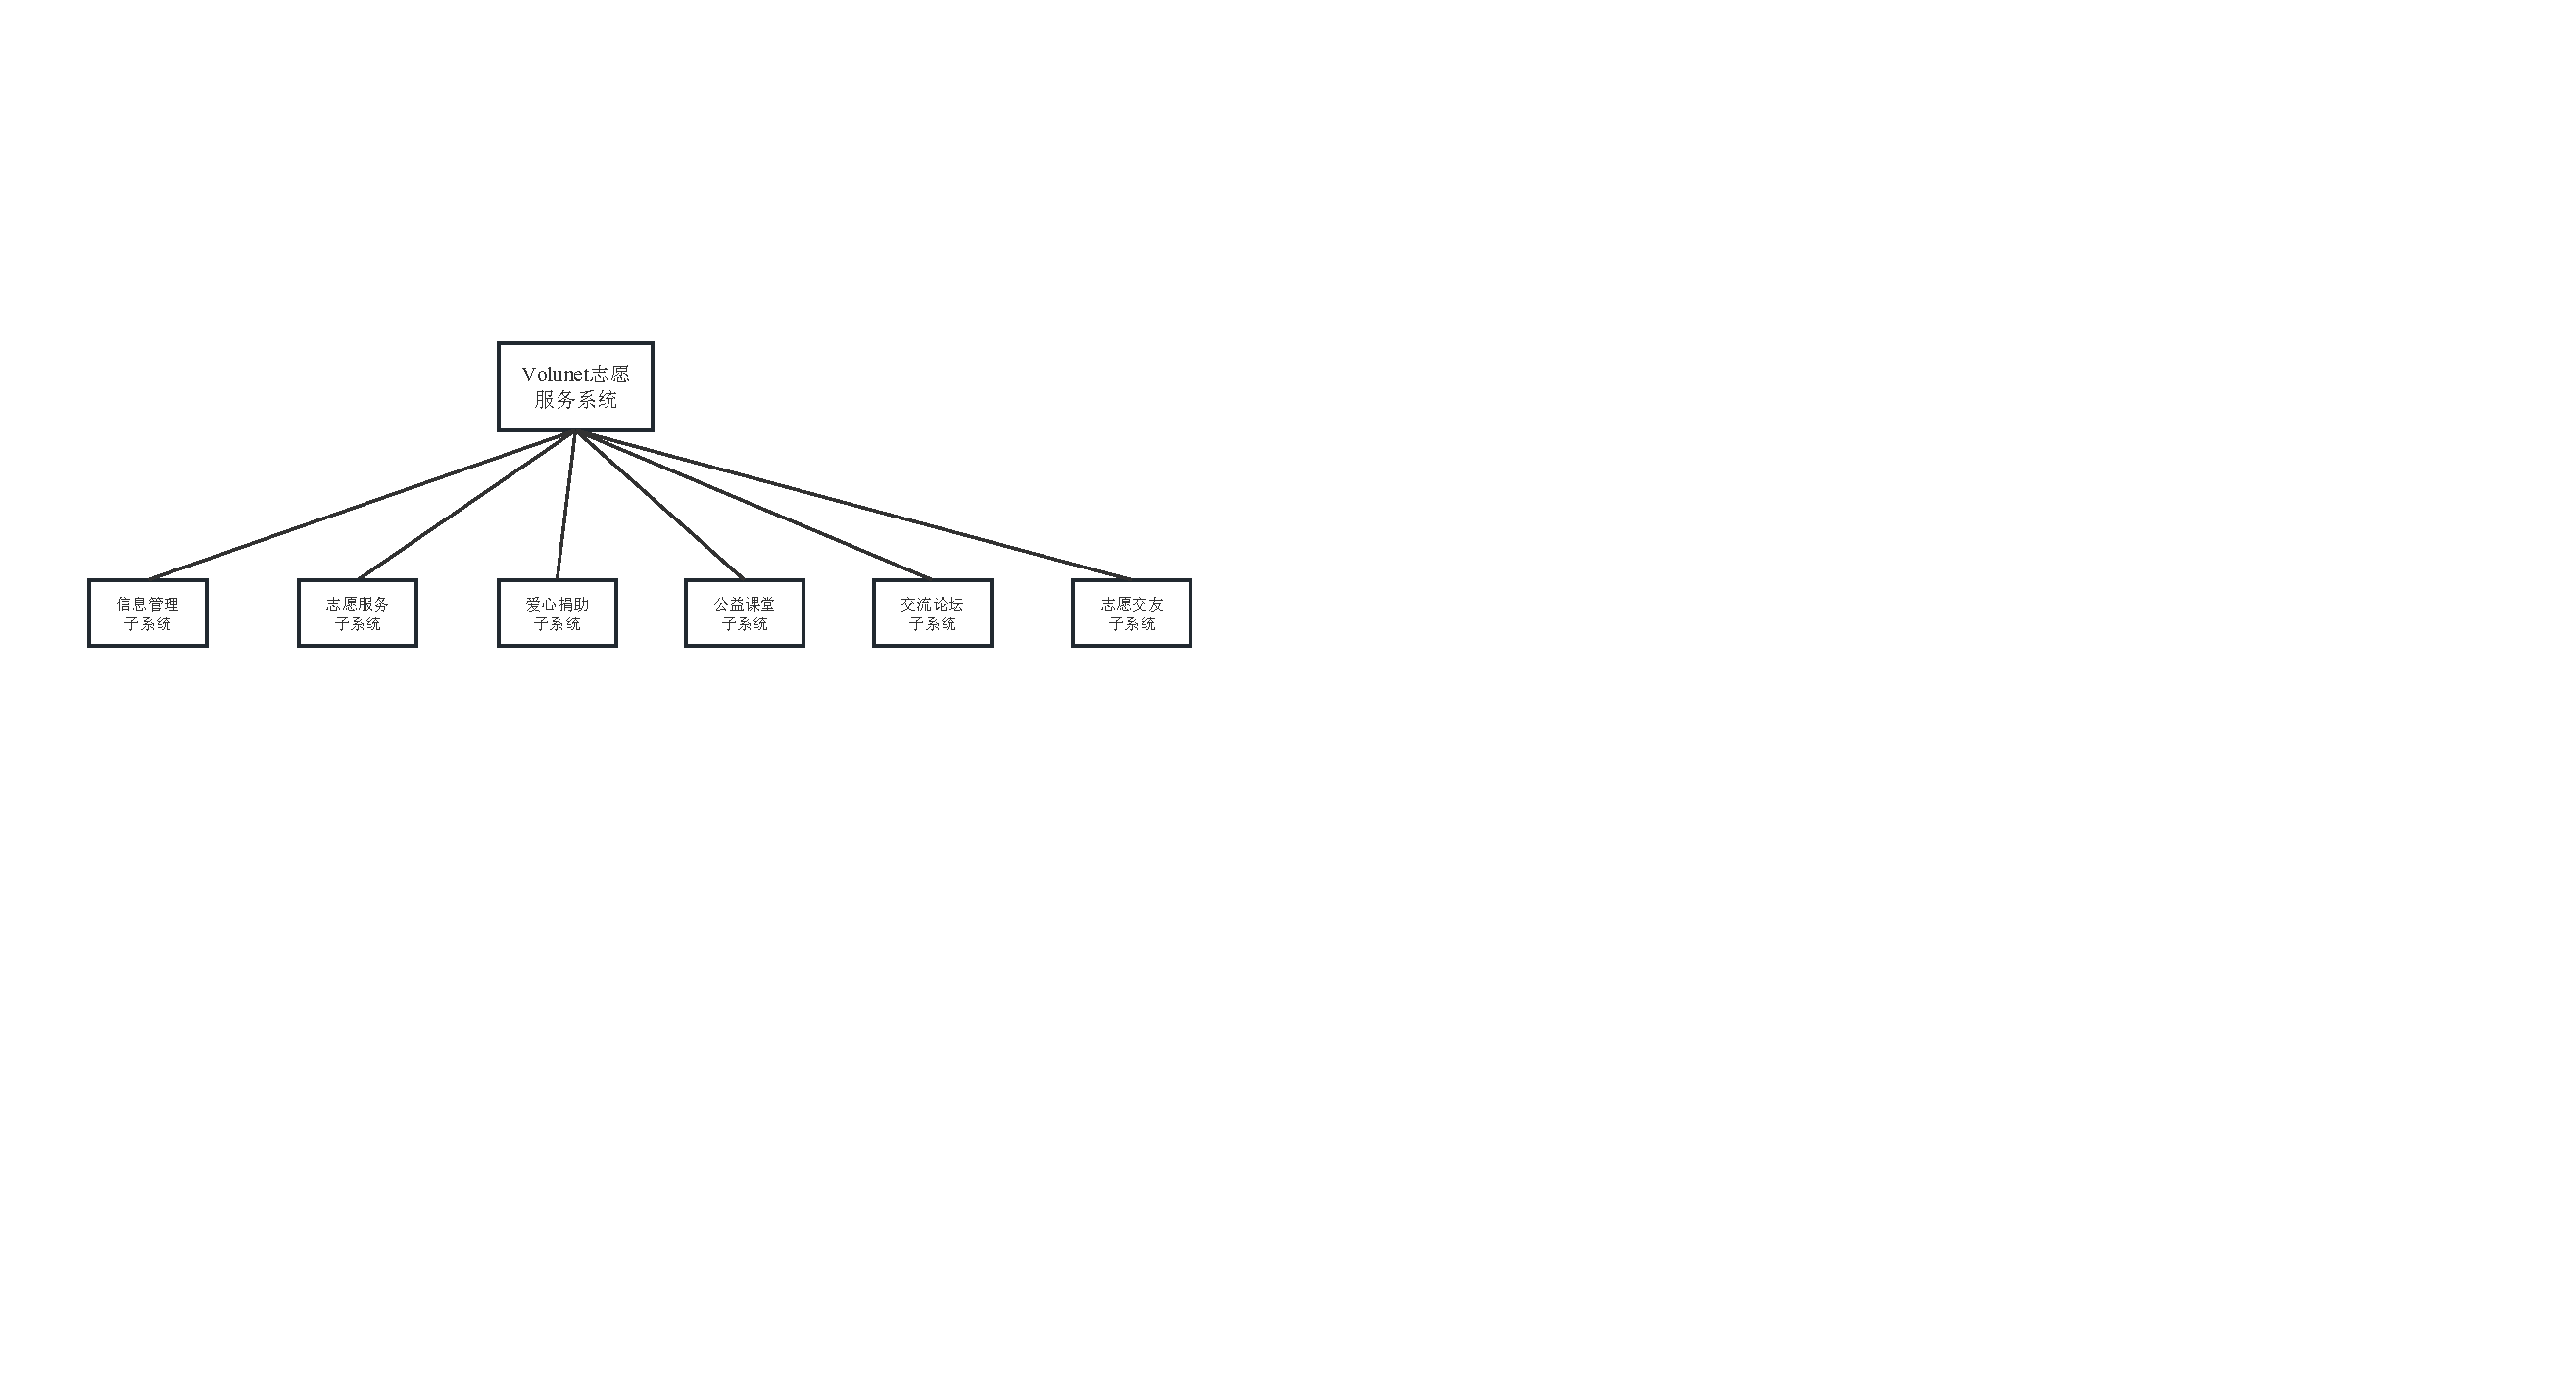
\includegraphics[scale=0.6]{fig/struct_0.pdf}
        \bicaption{Volunet志愿服务系统0层结构映射图}{Volunet Volunteer Service System Level 0 Structure Mapping Diagram}
        \label{fig:volunet}
    \end{figure}

0层映射将Volunet志愿服务系统划分为6个子系统:信息管理子系统、志愿服务子系统、爱心捐助子系统、公益课堂子系统、交流论坛子系统和志愿交友子系统。下一节将对每个子系统做进一步地拆解与分析,并在第三节给出完整的Volunet志愿服务系统结构图。

\subsection{分层结构图与设计说明}
\subsubsection{信息管理系统}



“信息管理系统”模块的主要目的是对Volunet志愿服务系统中用户团队信息相关的行为进行统一地管理。志愿者可以注册成为用户,系统会赋予用户权限,用户之后可以更新注册信息。用户登录时会收到反馈。志愿团队可以申请入驻,系统管理员进行审核,审核通过后正式入驻并通知志愿团队。系统管理员可以查询用户,修改用户权限。用户可以检索团队,据此申请加入团队,团队审核通过后通知到用户。

“信息管理系统”本身有五项职能,分别对应五个模块,详细如下:\\
1. 注册管理:基于加工1.1数据流图的变换型程序结构。逻辑输入端获取用户注册与更新信息,变换中心将用户信息转换为对应的注册反馈信息,逻辑输出端发送注册反馈信息。\\
2. 登陆填写与验证:基于加工1.2数据流图的变换型程序结构。逻辑输入端获取登录信息,变换中心将登录信息转换为对应的登录反馈信息,逻辑输出端发送登录反馈信息。\\
3. 团队管理:基于加工1.3数据流图的变换型程序结构。逻辑输入端获取团队基本信息,变换中心将团队基本信息转换为对应的入驻反馈信息,逻辑输出端发送入驻反馈信息。\\
4. 用户管理:基于加工1.4数据流图的变换型程序结构。逻辑输入端获取用户查询条件,变换中心获取查询结果并设置用户权限,逻辑输出端发送更新后用户信息。\\
5. 组队管理:基于加工1.5数据流图的变换型程序结构。逻辑输入端获取团队查询条件,变换中心获取查询结果并设置申请加入团队,逻辑输出端发送入队审核反馈。\\

\begin{landscape}
    \begin{figure}[bp]
        \center{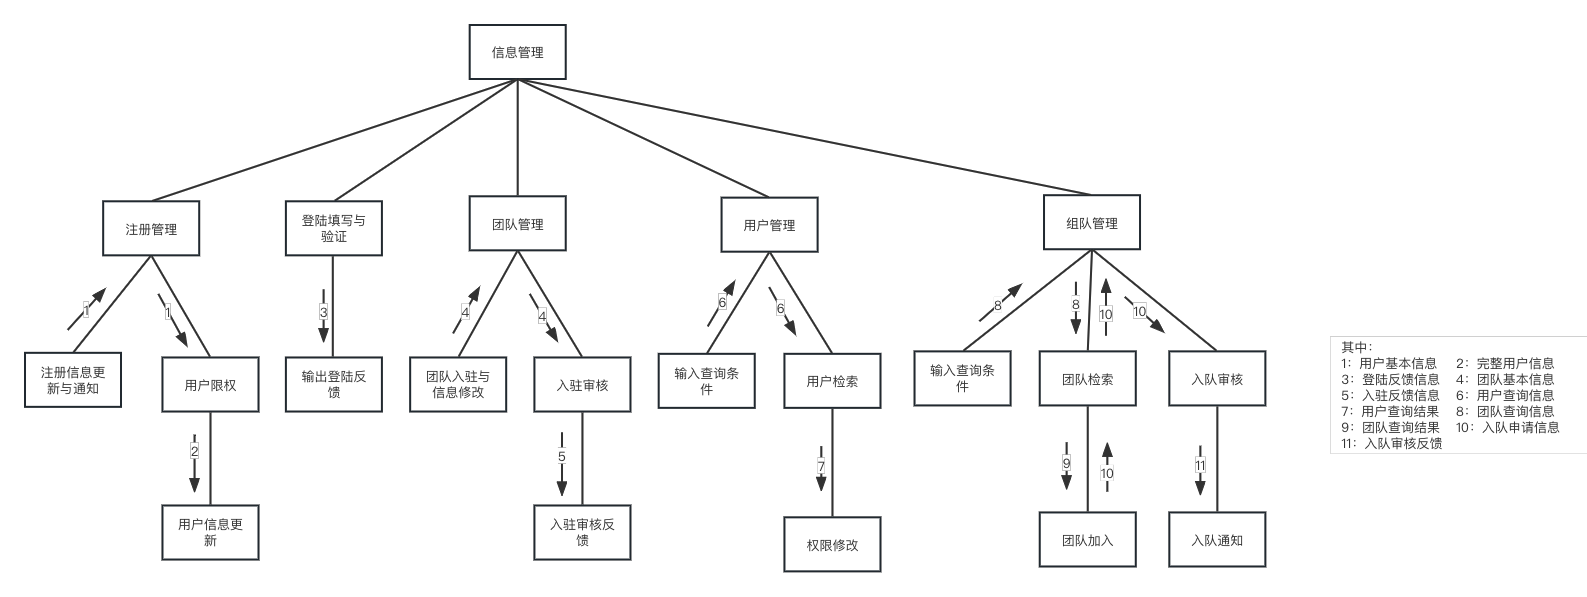
\includegraphics[scale=0.5]  {fig/信息管理/信息管理系统分解结构图.png}} 
        \bicaption{信息管理系统结构图}{Information Management System Structure Diagram}
        \end{figure}
\end{landscape}

\subsubsection{志愿服务系统}

“志愿服务系统”模块的主要目的是对Volunet志愿服务系统的志愿服务项目发布、项目报名参与和项目过程管理进行统一管理。该模块可以提供一个统一的平台,让志愿者和志愿者团队可以方便地进行志愿服务项目的参与与管理。志愿团队可以向Volunet提交项目申请单,在申请通过之后该项目会向志愿者用户推荐。志愿者根据自己的兴趣报名志愿项目,用户报名信息经过志愿团队筛选之后确认最终志愿者名单。在志愿项目进行的过程中,志愿者需要进行签到、签退进行记录,在活动结束之后对该项目进行评价。这些信息将生成活动反馈报告交由志愿者团队,同时部分信息也会在论坛发布,供其他用户了解。 

“志愿服务系统”本身有三项职能,分别对应三个模块,详细如下:\\
1. 项目发布:基于加工2.1数据流图的变换型程序结构。逻辑输入端获取志愿项目申请单,变换中心将申请单转换为正式项目信息表,逻辑输出端发送正式项目信息表。\\
2. 项目报名:基于加工2.2数据流图的变换型程序结构。逻辑输入端获取志愿者报名单,变换中心将志愿者报名单转换为入选志愿者信息表,逻辑输出端发送入选志愿者信息表。\\
3. 项目管理:基于加工2.3数据流图的变换型程序结构。逻辑输入端获取参与志愿者信息表、签到信息、签退信息、反馈评价,变换中心将输入信息转换为对应的活动情况报告,逻辑输出端发送活动情况报告。\\

\begin{landscape}
    %\Large This is a landscape page.
    \begin{figure}[bp]
    \center{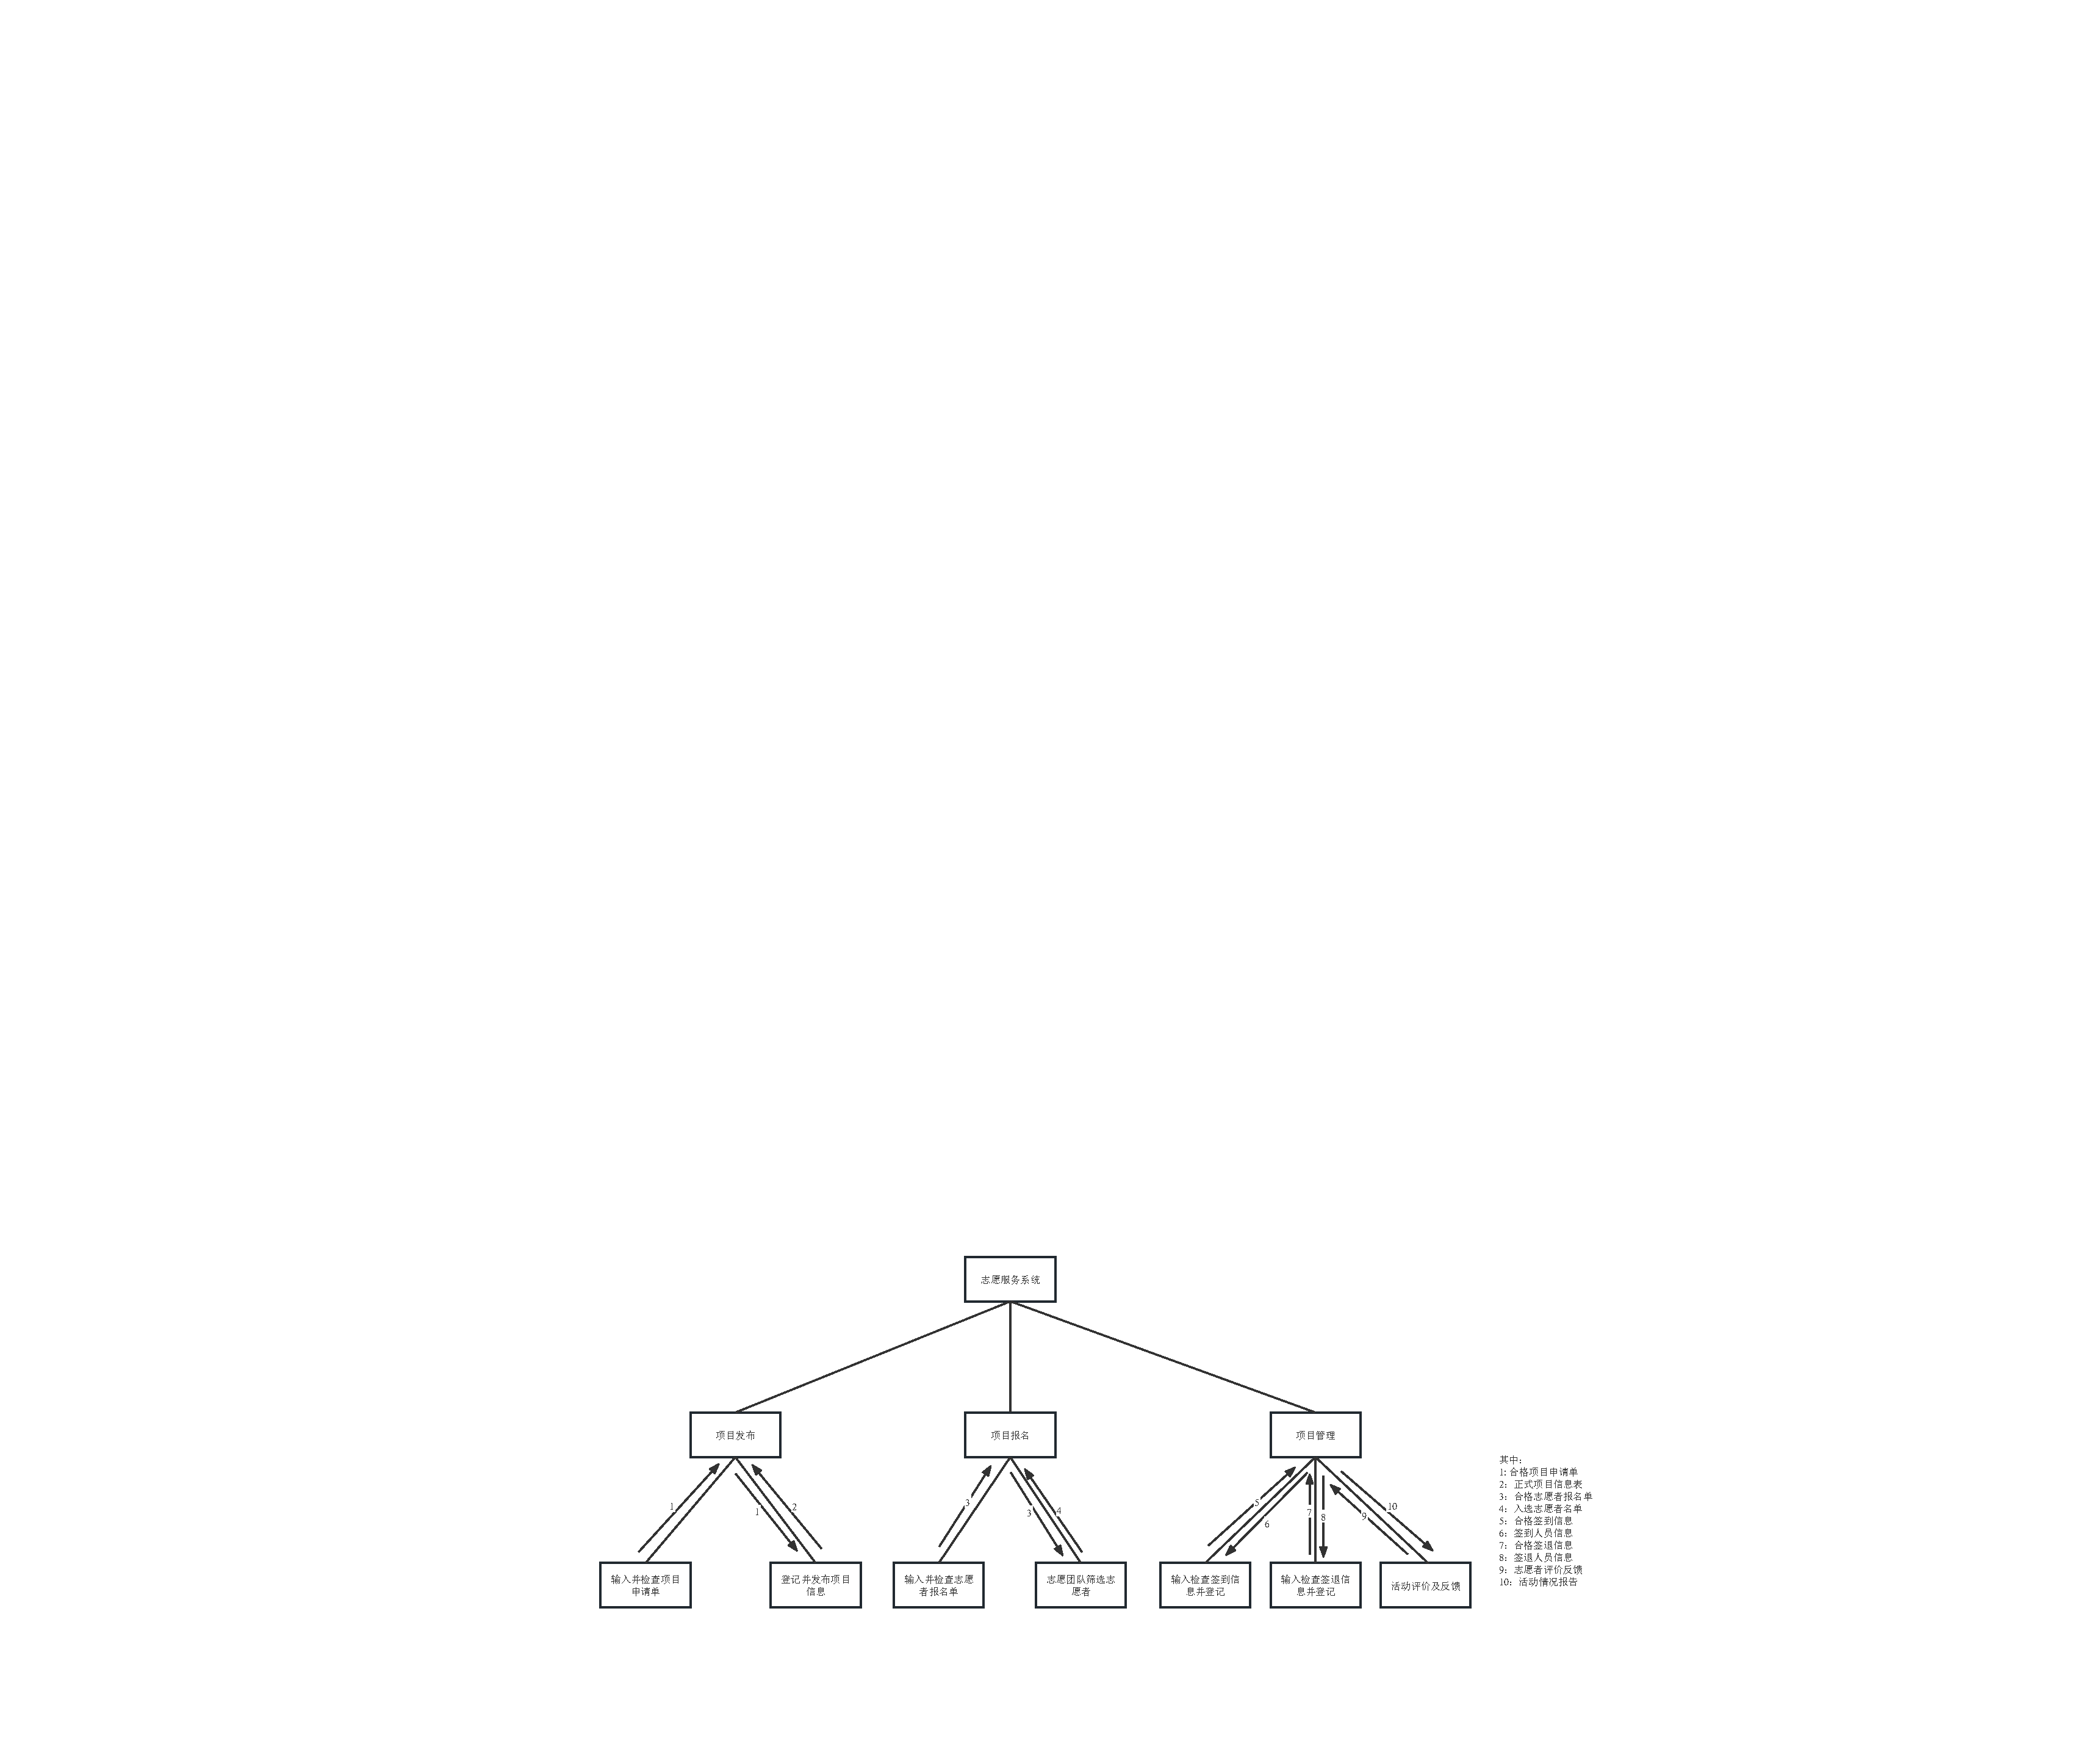
\includegraphics[scale=0.7] {fig/志愿服务/VS_S.pdf}} 
    \bicaption{志愿服务系统结构图}{Volunteer Service System Structure Diagram}
    \end{figure}

\end{landscape}



\subsubsection{爱心捐助系统}



“爱心捐助系统”模块的主要目的是对Volunet志愿服务系统的爱心商品的购买、公益项目的捐款等爱心捐助活动以及对爱心人士的反馈进行统一地管理。该模块可以提供一个统一的平台,让用户可以方便地进行爱心捐赠和爱心购物的活动。用户可以购买Volunet系统中的爱心商品,或者进行公益项目的捐款。这些捐赠活动的记录都会被统一记录和管理,方便管理员进行财务管理和透明度展示,并将审计报表交与有关部门以备复核。此外,该模块还可以提供给爱心人士一个反馈和感谢的渠道,让他们奉献的爱心能够得到及时的回馈和认可,增强他们的参与热情和对Volunet系统的信任度。

“爱心捐助系统”本身有三项职能,分别对应三个模块,详细如下:\\
1. 订单管理:基于加工3.1数据流图的变换型程序结构。逻辑输入端获取订单的状况信息,变换中心将订单信息转换为合格的订单信息、对应的快递信息以及购买者的爱心人士信息,逻辑输出端发送完结的订单信息和购买者的爱心人士信息。\\
2. 捐款管理:基于加工3.2数据流图的变换型程序结构。逻辑输入端获取项目信息和捐款资助明细,变换中心将项目信息和捐款信息转换为对应的打款信息和爱心人士信息,逻辑输出端发送爱心人士信息。\\
3. 爱心反馈管理:基于加工3.3数据流图的变换型程序结构。逻辑输入端获取爱心人士信息,变换中心将爱心人士信息转换为对应的爱心反馈信息,逻辑输出端发送爱心反馈信息。\\

\begin{landscape}
\begin{figure}[bp]
    \center{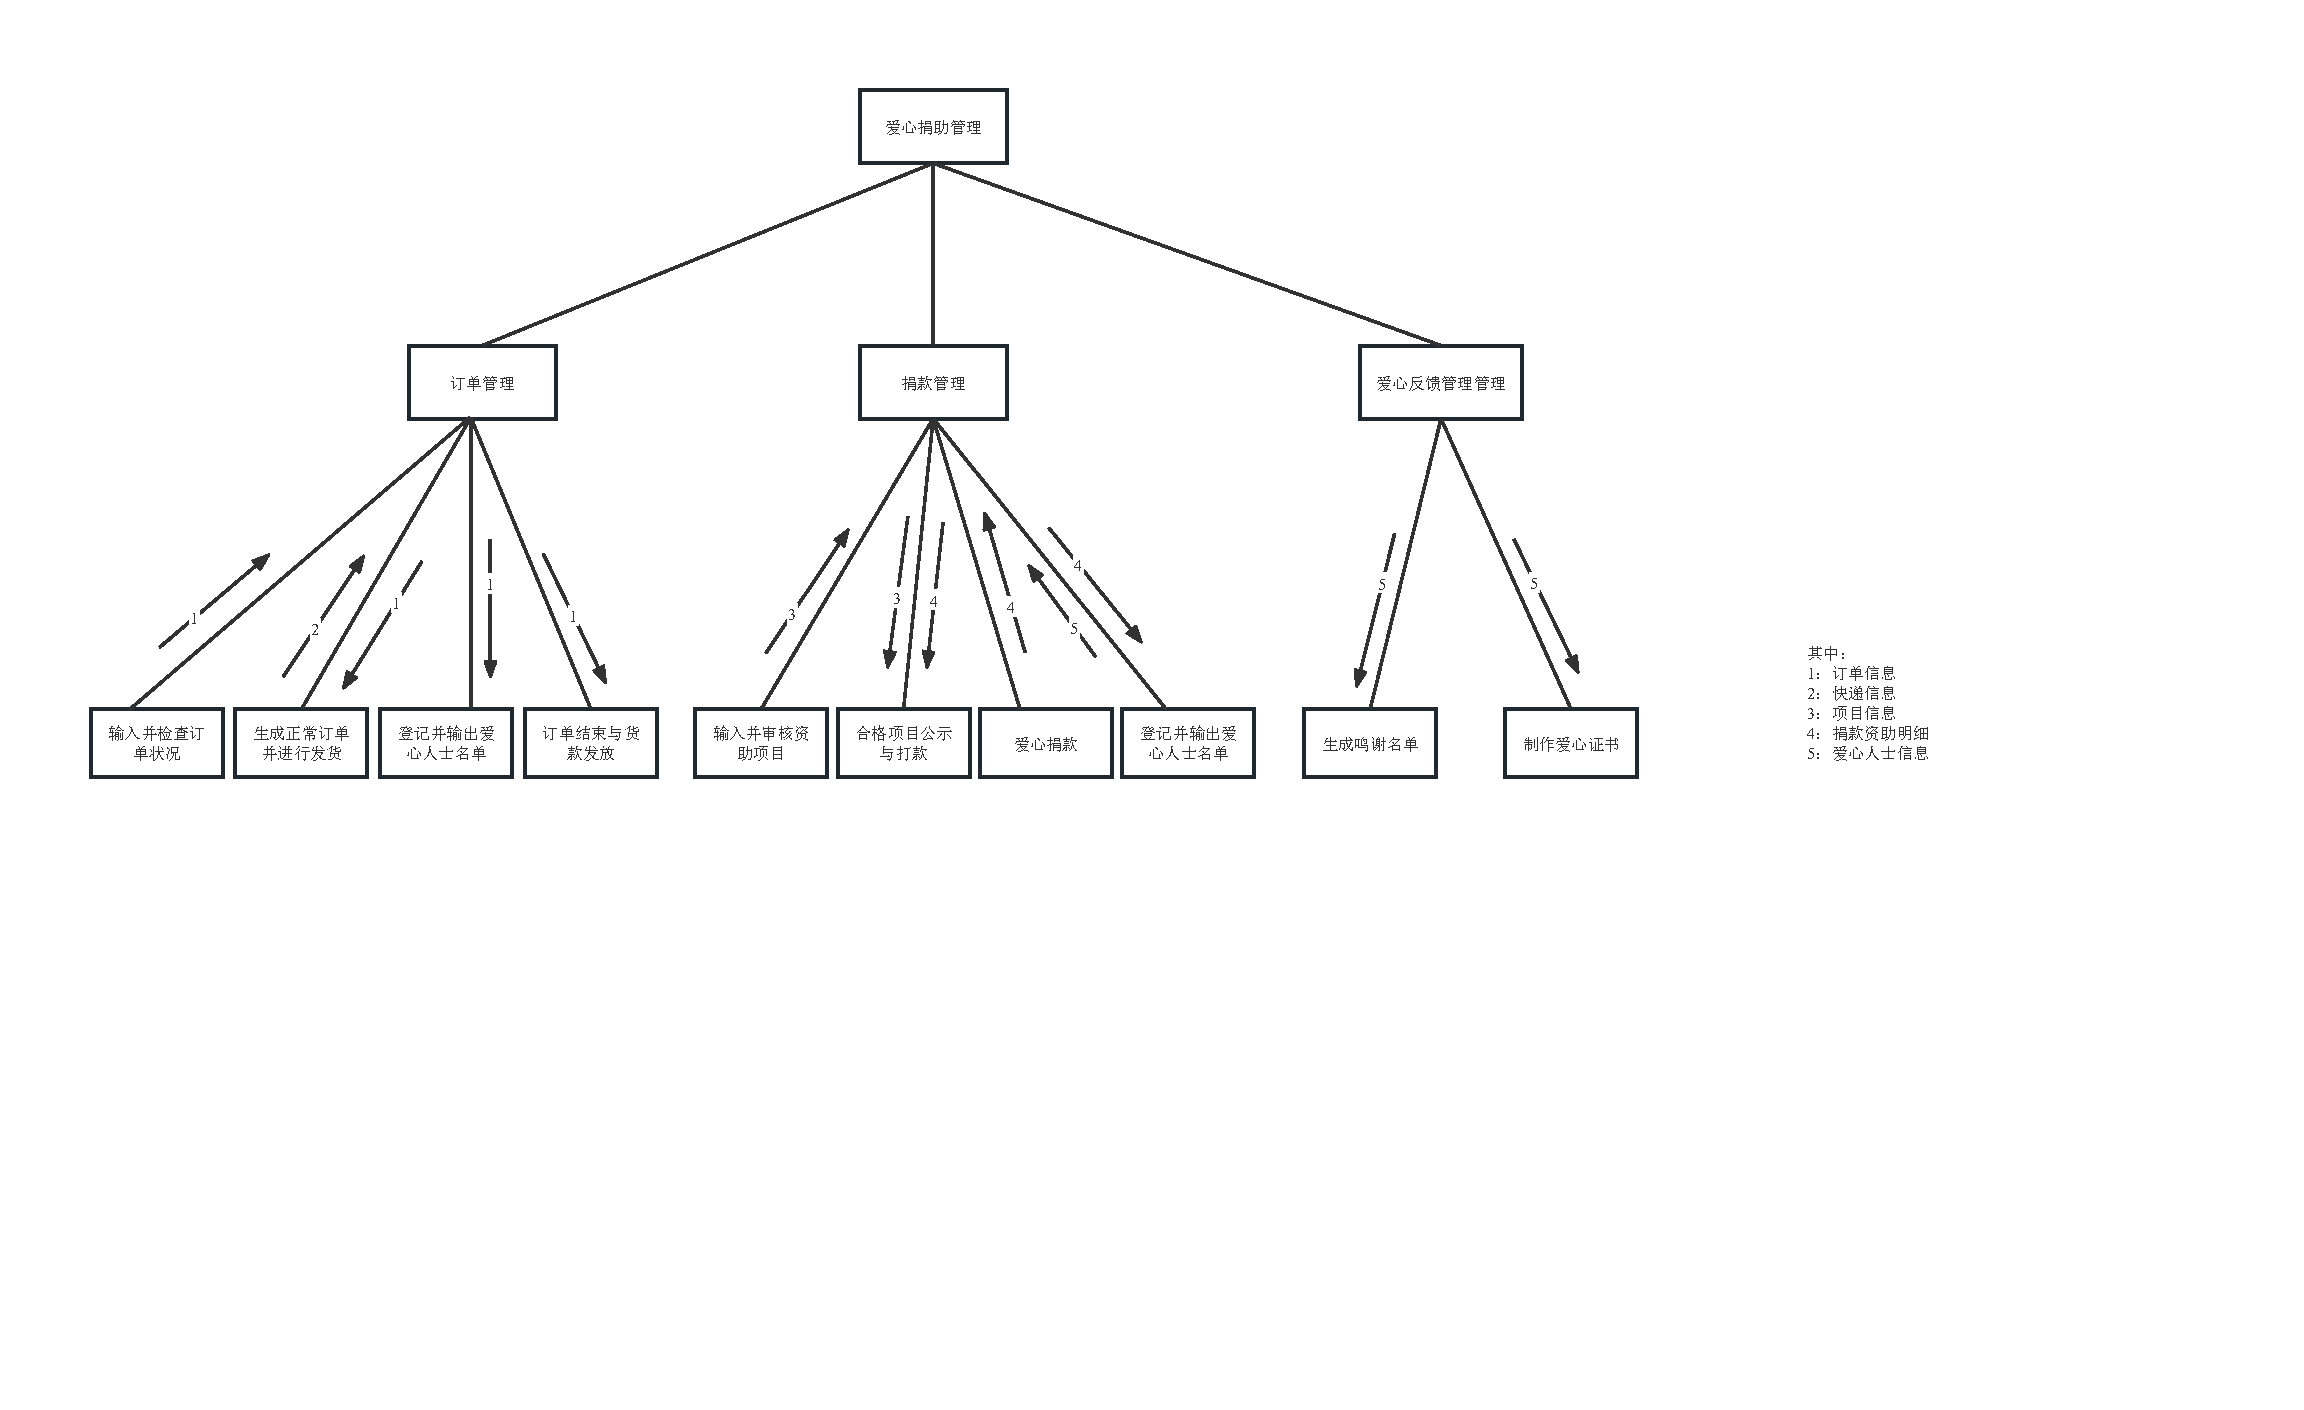
\includegraphics[scale=0.6]  {fig/爱心管理/C_S.pdf}} 
    \bicaption{爱心捐助系统结构图}{Love Donation System Structure Diagram}
    \end{figure}
\end{landscape}

\subsubsection{公益课程系统}

“公益课程系统”模块的主要目的是通过Volunet公益课程系统进行授课、学习,志愿者可以通过学习公益课程掌握更多的公益技能。该模块可以提供一个统一的平台,让授课人可以进行授课,志愿者可以方便地进行课程学习。授课人在提交授课申请通过之后,可以在Volunet开设自己的课程,并获得学生的课程参与情况及反馈。志愿者提交选课申请通过之后,学习相对应课程,在修读完成之后将获得结课证书。

通过对结构图的改进,我们将“公益课程系统”的四个模块(授课管理、修读管理、证书管理、反馈管理)合并为三个主要节点:授课管理、修读管理、反馈管理,详细如下:\\
1. 授课管理:基于加工4.1数据流图的变换型程序结构。逻辑输入端获取授课申请书、课程内容,变换中心将授课申请书、课程内容转换为课程信息,逻辑输出端发送学生修读情况。\\
2. 修读管理:基于加工4.2数据流图的变换型程序结构。逻辑输入端获取选课申请单和上课信息,变换中心将选课申请单和上课信息转换为对应的选课信息和学生修读情况,逻辑输出端发送学生修读情况。\\
3. 反馈管理:基于加工4.3数据流图的变换型程序结构。逻辑输入端获取课程反馈,变换中心将课程反馈转换为可输出的课程反馈,逻辑输出端发送课程反馈信息。\\

\begin{landscape}
\begin{figure}[bp]
    \center{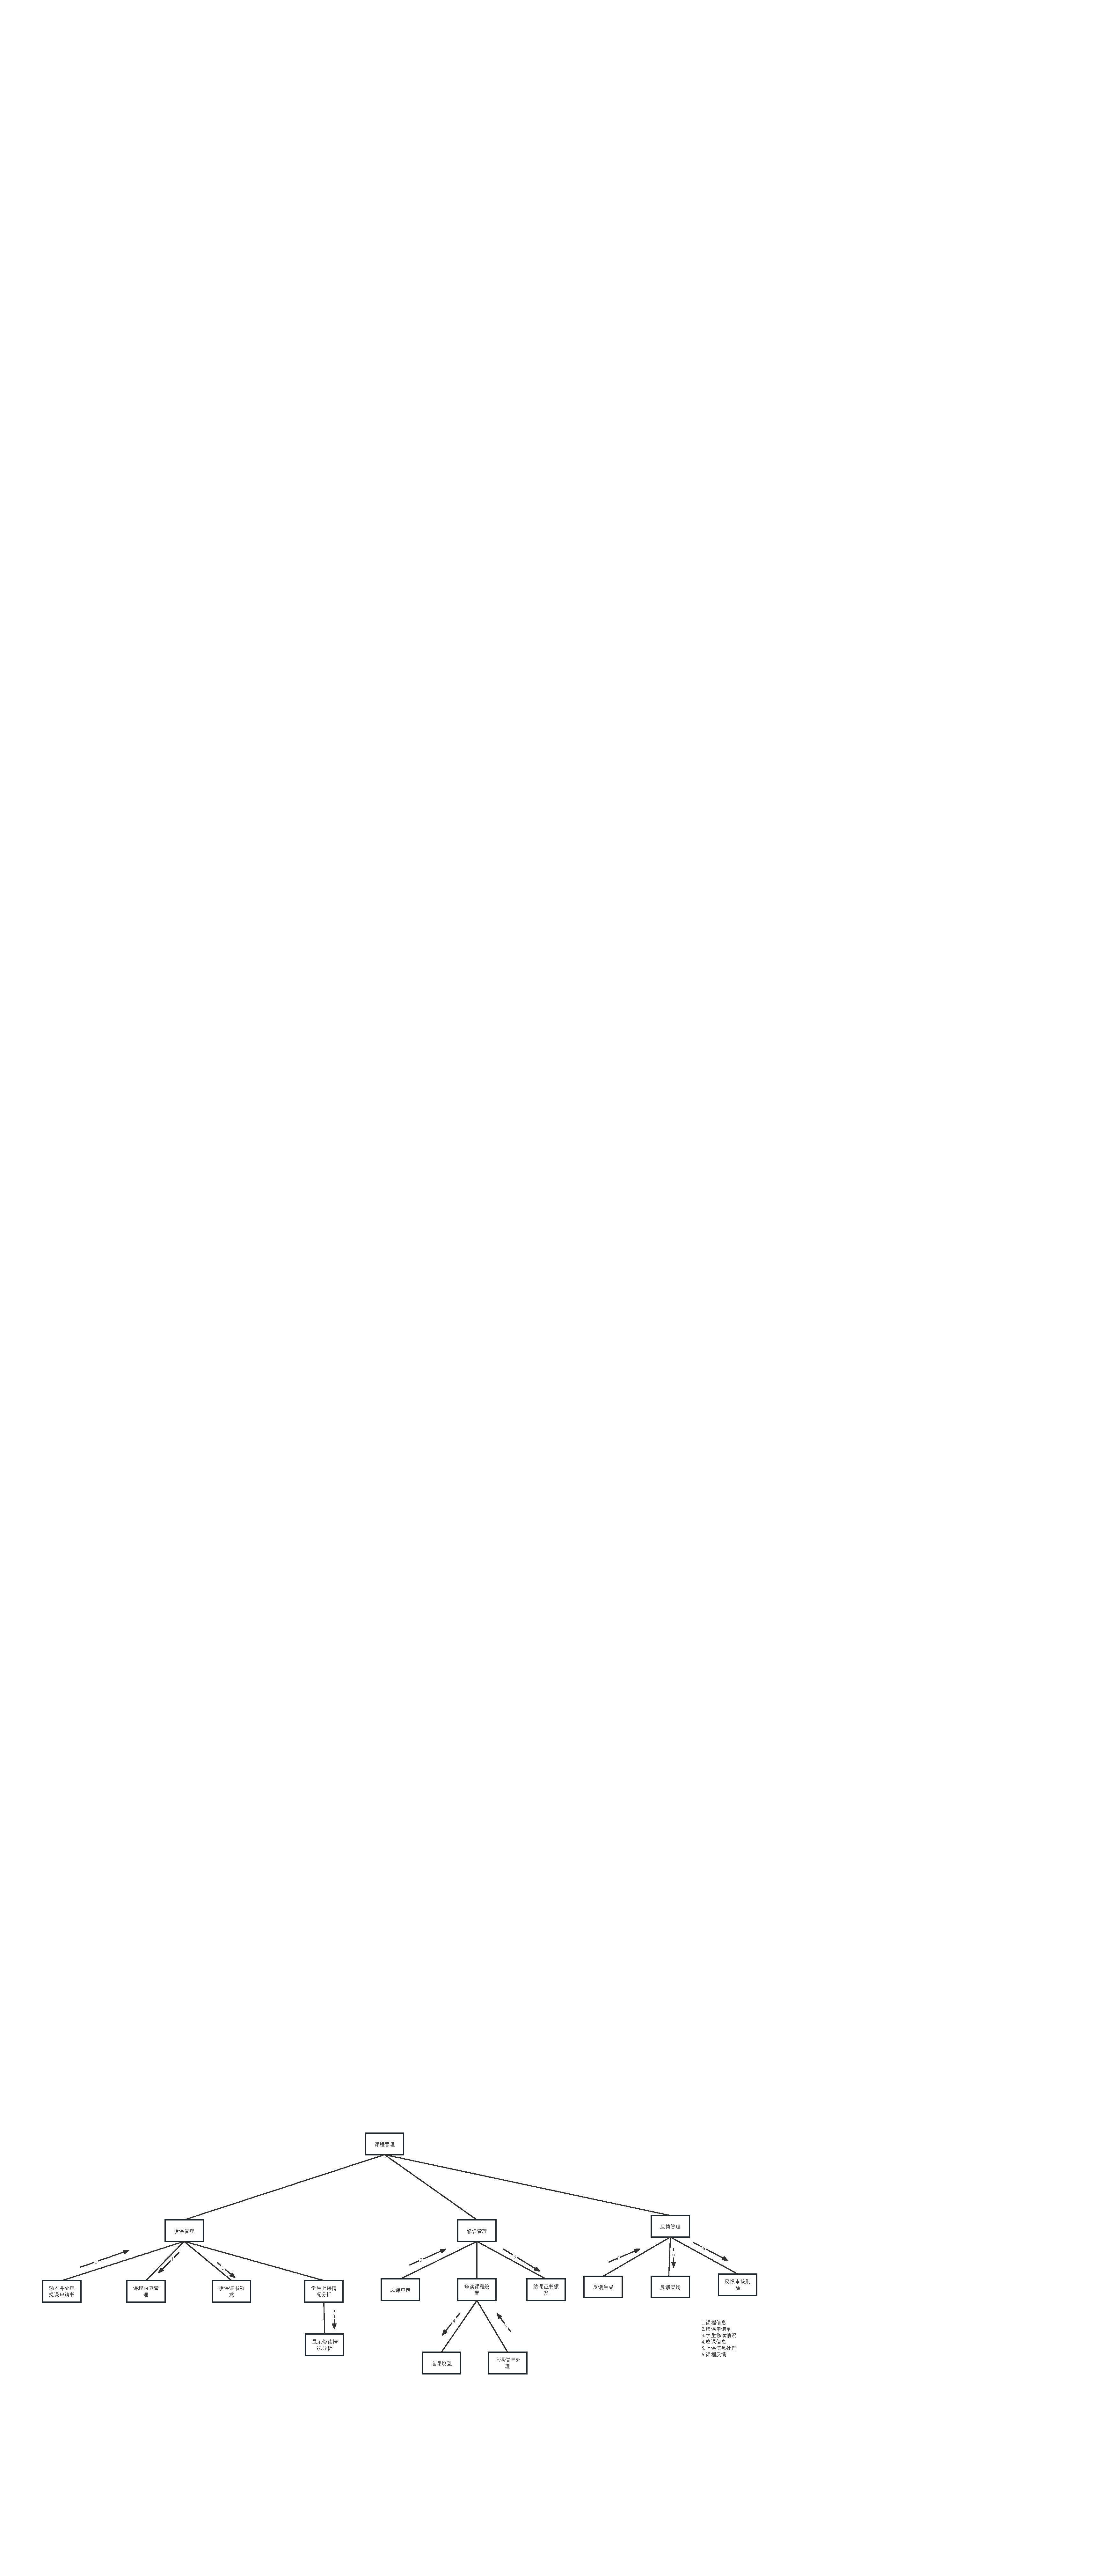
\includegraphics[scale=0.55]  {fig/课程管理/C_S.pdf}} 
    \bicaption{公益课程系统结构图}{Love Donation System Structure Diagram}
    \end{figure}
\end{landscape}

\subsubsection{交流论坛系统}



“交流论坛系统”模块的主要目的是对Volunet志愿服务系统中用户、团队、政府机构的资讯发布、用户的手记分享、用户发帖交流行为进行统一管理。志愿者、团队、政府机构均可通过系统发布资讯,发布者可以选择为资讯设定密码,系统根据内容为资讯设定分类。系统管理员审核资讯,提出修改意见,发布者必须据此进行修改。用户可以对资讯进行评论。系统会根据浏览情况和资讯内容,推送资讯给全体用户。系统会定期根据审核信息生成资讯审计报表,上报主管单位。用户可通过系统发布手记。系统管理员审核手记,提出修改意见,发布者必须据此进行修改。用户可以对资讯进行评论。系统会根据浏览情况和手记内容,推送手记给全体用户。系统会定期根据审核信息生成手记审计报表,上报主管单位。用户可在指定板块下发帖讨论版块话题相关的问题。系统管理员审核帖子,提出修改意见,发布者必须据此进行修改。用户可以订阅话题。系统会根据订阅情况,推送话题中帖子给用户。系统会定期根据审核信息生成帖子审计报表,上报主管单位。

“交流论坛系统”本身有三项职能,分别对应三个模块,详细如下:\\
1. 资讯管理:基于加工5.1数据流图的变换型程序结构。逻辑输入端获取编写好的资讯,变换中心设定资讯的密码和类别并审核修改,逻辑输出端发送筛选后的资讯给用户,发送审计报表给政府机构。\\
2. 手记管理:基于加工5.2数据流图的变换型程序结构。逻辑输入端获取编写好的手记,变换中心审核修改手记,逻辑输出端推送筛选处理后的手记给用户,发送审计报表给政府机构。\\
2. 交流管理:基于加工5.3数据流图的变换型程序结构。逻辑输入端获取编写好的帖子,变换中心设定帖子所属话题并审核修改,逻辑输出端推送筛选处理后的后的帖子给用户,发送审计报表给政府机构。

\begin{landscape}
\begin{figure}[bp]
    \center{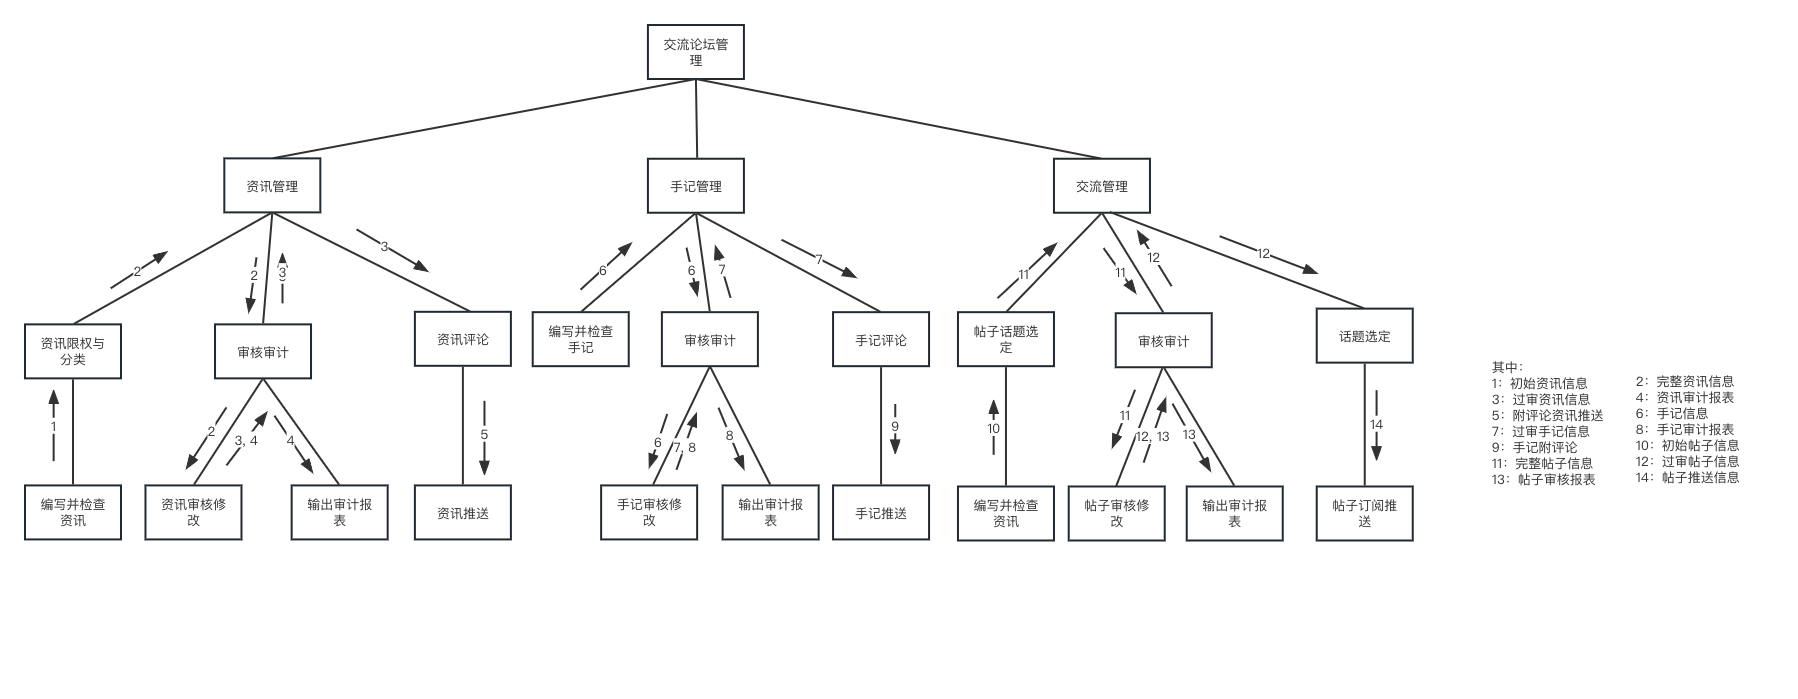
\includegraphics[scale=0.3]  {fig/论坛管理/交流论坛管理分解结构图.png}} 
    \bicaption{交流论坛系统结构图}{Communication Forum System Structure Diagram}
    \end{figure}
\end{landscape}

\subsubsection{志愿交友系统}

“志愿交友系统”模块的主要目的是对Volunet志愿服务系统中用户的交友,私聊行为进行统一地管理。用户可以输入关键词检索其他用户,并据此申请添加好友,被添加者可以同意亦可拒绝。对于已经互为好友的一对用户,两人可以互相发送消息。

“志愿交友系统”本身有两项职能,分别对应两个模块,详细如下:\\
1. 交友管理:基于加工6.1数据流图的变换型程序结构。逻辑输入端获取用户查询条件,变换中心获取查询结果并添加对应好友,发送端输出好友添加请求的反馈给用户。\\
2. 消息管理:基于加工6.2数据流图的事务型程序结构。接收端输入好友聊天消息,以信息管理为主控,发送端输出筛选处理之后的好友聊天消息。

\begin{landscape}
\begin{figure}[bp]
    \center{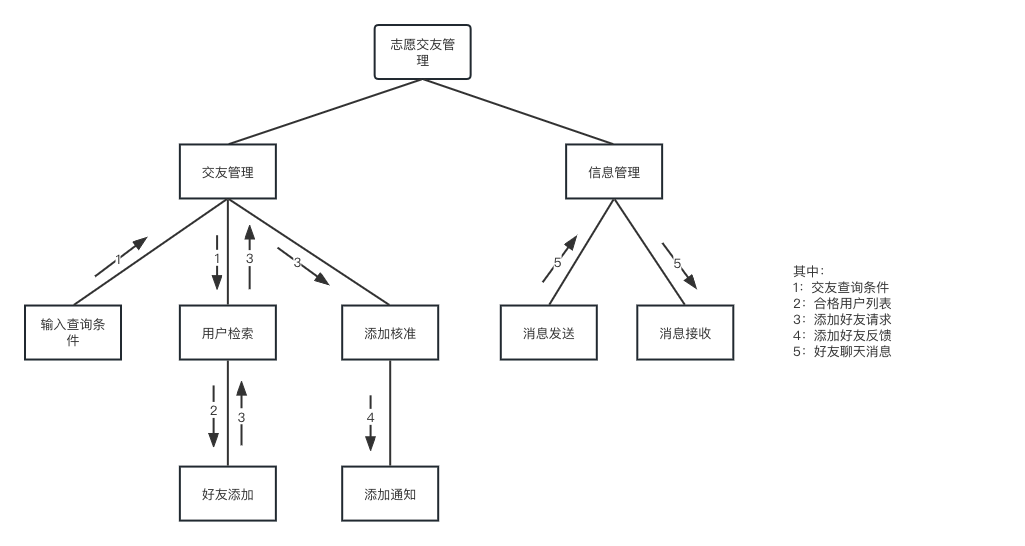
\includegraphics[scale=0.6]  {fig/社交管理/志愿交友管理分解结构图.png}} 
    \bicaption{志愿交友系统结构图}{Volunteer Social System Structure Diagram}
    \end{figure}
\end{landscape}

\subsection{总结构图}


\begin{figure}[H]
    \center{
\includegraphics[scale=0.08]{fig/struct_top.pdf}} 
    \bicaption{Volunet志愿服务系统结构图}{Volunet Volunteer Service System Structure Diagram}
    \end{figure}
